\documentclass{article}
\usepackage{graphicx} % Required for inserting images
\graphicspath{{Images/}}
\usepackage[utf8]{inputenc}
\usepackage{multicol}
\usepackage{amsthm}
\usepackage{amsmath}
\usepackage{xcolor}

\newtheorem{definition}{Definition}[section]
\newtheorem{remark}{Remarque}[section]
\newtheorem{theorem}{Théorème}

\title{Analyse I}
\author{Laura Paraboschi / Simon Lefort }
\date{BA1 - IN}

\begin{document}

\maketitle

\section{Règles de calcul}

\begin{multicols}{2}
\subsection{Puissance}  
\columnbreak
\subsection{Logarithme}
\end{multicols}

\begin{multicols}{2}

\begin{itemize}
    \item \( a^n \cdot a^m = a^{m+n} \)
    \item \( (ab)^m = a^mb^m \)
    \item \( (\frac{a}{b})^m = (\frac{a^m}{b^m}) \)
    \item \( \frac{a^m}{a^n} = a^{m-n} \)
\end{itemize}
\columnbreak

\begin{itemize}
    \item \( \log_a(x \cdot y) = \log_a(x) + \log_a(y) \)
    \item \( \log_a(\frac{1}{x}) = -\log_a(x) \)
    \item \( \log_a(\frac{x}{y}) = \log_a(x) - \log_a(y) \)
    \item \( \log_a(x^r) = r\log_a(x) \)
\end{itemize}

\end{multicols}

\section{Ensemble}
\begin{definition}
P(X) est l'ensemble dont les éléments sont tous les sous-ensembles de X. Sa capacité est de  \(2^n\), avec n = nombres d'élements dans X
\end{definition}
\subsection{Produit cartésien}
\[ X \times Y \times Z := \{\,(x,y,z)\quad |\quad x \in X,\,y \in Y,\, z \in Z\, \} \]
\begin{definition}
    Un sous ensemble \(R \subset X \times Y\) est appelé \underline{une relation binaire} sur X et Y
\end{definition}
\begin{definition}
    Un sous ensemble \(R \subset X \times X\) est appelé \underline{une relation} sur X
\end{definition}

\subsection{Classe d'équivalence}
\begin{definition}
    Un sous ensemble \(R \subset X \times X\) est appelé \underline{une relation d'équivalence} sur X si :
    \begin{enumerate}
        \item \( \forall x \in X,\quad x \sim x \) (R est réfléctive)
        \item \( \forall x,\,y \in X,\quad  x \sim y \Rightarrow y \sim x \) (R est symétrique)
        \item \( \forall x,\,y,\, z \in X,\quad x \sim y\, \wedge\, y \sim z \Rightarrow x \sim z \) (R est transitive)
    \end{enumerate}
\end{definition}
\begin{definition}
    On définit \(C_x \subset X \) par \\ \[ C_x := \{\, y \in X\quad |\quad y \sim x\, \} \] \\
    \(C_x\) est appelé la classe d'équivalence de x
\end{definition}
\begin{definition}
    L'ensemble quotient \(X/_\sim \) est l'ensemble des classes d'équivalences distinctes de X
\end{definition}
\subsection{Fonction}
\begin{definition}
    Une fonction f : \(D \rightarrow Y\) est appelée 
    \begin{itemize}
        \item \underline{surjective} si Im(f) = Y
        \item \underline{injective} si \( f(x_1) = f(x_2) \Rightarrow x_1 = x_2 \)
    \end{itemize}
\end{definition}
\begin{remark}
    \( (A \Rightarrow B) \Leftrightarrow (\overline{A} \Rightarrow \overline{B}) \) \quad Une proposition contraposée
\end{remark}
\begin{remark}
    Toute fonction f : \(D \rightarrow Y\) définit une fonction surjective\\ \[f : D \rightarrow Im(f) \subset Y\]
\end{remark}
\begin{definition}
    Une fonction qui est surjective et injective est appelée bijective
\end{definition}
\begin{remark}
    Toute fonction bijective \(D \rightarrow Y\) possède une fonction réciproque notée \( f^{-1}, Y \rightarrow D\)
\end{remark}
Soient deux fonctions f :\(D \rightarrow Y\) et g : \(E \rightarrow Y\) avec \(E \subset D\), telle que pour tout \(x \in E, g(x) = f(x)\). Alors :
\begin{itemize}
    \item g est appelée la restriction de f à E : \(g = f|_E\)
    \item f est appelée un prolongement de g de E à D
\end{itemize}
\begin{definition}
    Le graphe d'une fonction f : \(D \rightarrow Y\) est l'ensemble
    \[ G_f := \{\, (x,y) \in D \times Y\quad |\quad y = f(x)\, \} \]
    \qquad Attention, pour tout x, il ne doit exister \textcolor{red}{qu'une seule} image (qu'un seul y = f(x)).
\end{definition}
\begin{definition}
    On définit \(h = g \circ f\) comme étant la composition de fonction 
    \[h = g(f(x))\]
    \qquad La loi de la composition de fonction est associative
\end{definition}
\newpage
\section{Plus grand commun diviseur}
\subsection{Algorithme de J. Stein}
\begin{itemize}
    \item pgcd(a,b) = pgcd(b,a)
    \item pgcd(a,b) = 2\(\cdot\) pgcd(\(\frac{a}{2},\frac{b}{2})\) \qquad si a, b pairs
    \item pgcd(a,b) = pgcd(\(\frac{a}{2}\),b) \qquad si a pair, b impair
    \item  pgcd(a,b) = pgcd(\(\frac{a-b}{2}\), b)  \qquad si a, b impairs et a \(\geq \) b
    \item pgcd(a,0) = a
\end{itemize}
\section{Raisonnement par récurrence}
\begin{theorem} 
\end{theorem}
\begin{enumerate} 
    \item Si P(\(n_0)\) est vrai pour un \(n_0 \in \mathbf{N}\)
    \item Si pour tout n \(\geq n_0\), P(n) \(\Rightarrow\) P(n+1)
\end{enumerate}
\qquad \textit{Alors P(n) est vrai pour tout n \(\geq n_0\)}
\section{Les notations \(\Sigma\) et \(\Pi\)}
\(\sum_{k=m}^n a_k := a_m + a_{m+1} + ... + a_{n-1} + a_n \) \\\\
\( \prod_{k=m}^{m} a_k := a_m \cdot a_{m+1} \cdot ... \cdot a_{n-1} \cdot a_n\)\\\\
\( Si\ n < m, alors \qquad \sum_{k=m}^{n} a_k := 0,\qquad \prod_{k=m}^{n} a_k = 1 \)
\subsection{Règles de calcul}
\( \sum_{k=l}^{m} a_k + \sum_{k=m+1}^{n} a_k = \sum_{k=l}^{n} a_k \)\\\\
\( (\prod_{k=l}^{m} a_k)\cdot(\prod_{k=m+1}^{n} a_k) =\prod_{k=l}^{n} a_k \)\\\\
\( \sum_{k=m}^{n}(a_k + b_k) = \sum_{k=m}^{n} a_k + \sum_{k=m}^{n} b_k \)\\\\
\( \prod_{k=m}^{n}(a_k \cdot b_k) = (\prod_{k=m}^{n} a_k) \cdot (\prod_{k=m}^{n} b_k)\)
\subsection{Identité}
\(\sum_{k=0}^{n} a^k = \frac{1-a^{n+1}}{1-a}, \qquad a \neq 1\)\\\\
\( \sum_{k=0}^{n} k = \frac{n\cdot(n+1)}{2} \)\\\\
\( (a + b)^2 = a^2 + 2ab + b^2  \)\\\\
\( (a + b)^3 = a^3 + 3a^2b + 3ab^2 + b^3 \)\\\\
\( (a + b)^n = \sum_{k=0}^{n} 
\begin{pmatrix}
    n \\ k
\end{pmatrix} a^{n-k}\cdot b^k = a^n + na^{n-1}b + ... + b^n \)\\\\
On peut tout déduire du triangle de Pascal :
\begin{figure}[htp]
    \centering
    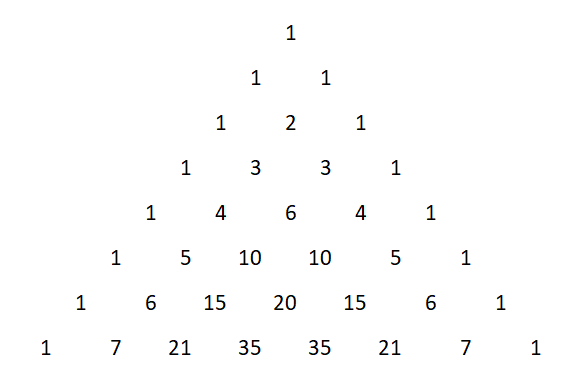
\includegraphics[width=8cm]{Images/Pascal-Triangle.png}
    \caption{Triangle de Pascal}
\end{figure}
\section{Nombres réels}
\begin{definition}
Un corps est un ensemble muni des opérations + et $ \cdot $, rendant possible le calcul d'opposés et d'inverses
\end{definition}
\begin{definition}
    R est un corps qui a les propriétés suivantes :
    \begin{multicols}{2}
        
    
    \begin{itemize}
        \item x + (y + z) = (x + y) + z
        \item x + y = y + x
        \item 0 + x = x
        \item (-x) + x = 0 
        \columnbreak
        \item \( x \cdot (y \cdot z) =  (x \cdot y) \cdot z\)
        \item \( x \cdot y = y \cdot x\) 
        \item  \(1 \cdot x = x \)
        \item \( x^{-1} \cdot x = 1\)
        \item \(x \cdot (y + z) = x \cdot y + x \cdot z\)
    \end{itemize}
    \end{multicols}
    Un corps \underline{ordonné} est en plus compatible avec \( \leq \) 
\end{definition}
\begin{definition}
    Un corps archimédien a la propriété suivante :\\
    Pour tout x, y \(\in\) au corps, x \(>\) 0, y \(\geq\) 0 il existe n \(\in N^*\) tel que nx \(>\) y
\end{definition}
Les démonstrations peuvent être faites de plusieurs manières différentes :
\begin{itemize}
    \item Raisonnement déductif : Si A est vrai et A \(\implies\) B, alors B est vrai
    \item Raisonnement par l'absurde : Si B est vrai et A \(\implies \overline{B}\), alors \(\overline{A}\) est vrai
\end{itemize}
\subsection{Infimum et Supremum}
\underline{minimum} : plus petite valeur de A \\
\underline{maximum} : plus grande valeur de A \\
\underline{minorant} : a \(\leq\) x, a appartenant à R, x appartenant à A \\ infimum (ou borne inférieure) si a est le plus grand minorant \\\\
\underline{majorant} : x \(\leq\) a, a appartenant à R, x appartenant à A  \\ suprémum (ou borne supérieure) si a est le plus petit majorant\\\\
\underline{minoré} : A admet un minorant \\
\underline{majoré} : A admet un majorant \\
\underline{borné} : A admet un minorant et un majorant
\begin{remark}
    Un majorant/minorant peut être un maximum/minimum s'il appartient à A
\end{remark}
\subsection{Valeur absolue}
Inégalités triangulaires :
\begin{itemize}
    \item \( |x \pm y| \leq |x| + |y| \)
    \item \( |x \pm y| \geq ||x| - |y|| \)
\end{itemize}
Identités :
\begin{itemize}
    \item \( |x +\ y| + |x -\ y| =  |x| + |y| + ||x| - |y|| = 2 \cdot max\{|x|, |y|\}\)
    \item \( ||x +\ y| - |x -\ y|| =  |x| + |y| - ||x| - |y|| = 2 \cdot min\{|x|, |y|\}\)
\end{itemize}
\section{Nombres complexes}
\begin{definition}
   \( \mathbf{C} = (X, +, \cdot) \qquad X = \mathbf{R} \times \mathbf{R} \)\\\\
   \( + : (a, b) + (c, d) = (a + c,\ b + d)\) \\\\
   \( \cdot : (a, b) \cdot (c, d) = (ac - bd,\ ad + bc) \)
\end{definition} \newpage
\subsection{Représentation cartésienne}
\begin{figure}[htp]
    \centering
    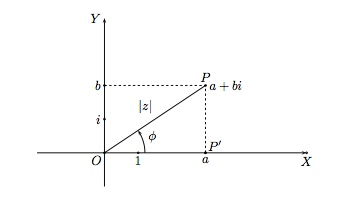
\includegraphics[width=12cm]{Images/complexe2.jpeg}
    \caption{Représentation des nombres complexes}
    \label{fig:complex}
\end{figure} 
\underline{Notations :} 
\begin{itemize}
    \item i = (0,1) et \(i^2\)= -1 (-1, 0), c'est l'unité imaginaire 
    \item z = a + ib, \qquad \qquad \qquad \qquad avec a = Re(z) = \( \frac{z + \overline{z}}{2}\) et b = Im(z) = \( \frac{z - \overline{z}}{2}\)
\end{itemize}
\subsection{Définitions additionelles}
\begin{figure}[htp]
    \centering
    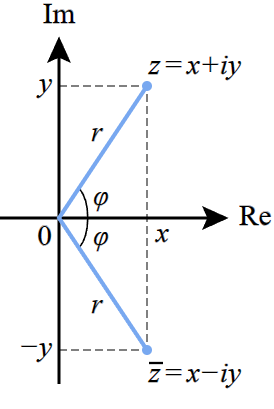
\includegraphics[height=4cm]{Images/conjugue.png}
    \label{fig:conjugue}
\end{figure}
Le \underline{complexe conjugué} de z : \( \overline{z} = a - ib\) \\
\begin{itemize}
    \item \( \overline{\overline{z}} = z \)
    \item \( \overline{z_1 + z_2} = \overline{z}_1+ \overline{z}_2 \)
    \item \( \overline{z_1 \cdot z_2} = \overline{z}_1 \cdot \overline{z}_2 \)
\end{itemize} \newpage
Le \underline{module} de z : \(|z| = (z\cdot\overline{z})^{\frac{1}{2}} = \sqrt{z\cdot\overline{z}} = \sqrt{a^2 + b^2} = |\overline{z}|\)
\begin{itemize}
    \item \( |z_1 \cdot z_2| = |z_1|\cdot|z_2| \)
\end{itemize}
L'\underline{élément inverse} de z : \(\frac{1}{z} = \frac{1}{|z|^2}\cdot\overline{z}\)
\begin{itemize}
    \item \(Re(\frac{1}{z}) = \frac{a}{a^2 + b^2}, \ Im(\frac{1}{z}) = \frac{-b}{a^2 + b^2} \)
    \item \( \frac{z_1}{z_2} = z_1 \cdot \frac{1}{z_2} \)
\end{itemize}
\underline{Formule d'Euler}
\[ e^{i\phi} = \cos{\phi} + i\sin{\phi} \]
\[ e^{z_1} \cdot e^{z_2} = e^{z_1 + z_2} \]
\[ \overline{e^z} = e^{\overline{z}} \]
\[ (e^z)^n = e^{n\cdot z} \]
\underline{Formule de Moivre}
\[ \cos{n\phi} + i\sin{n\phi} = (\cos{\phi} + i\sin{\phi})^n \]
\begin{itemize}
    \item \( \cos{\phi} = \frac{e^{i\phi} + e^{-i\phi}}{2} \Rightarrow \cos{z} = \frac{e^{iz} + e^{-iz}}{2} \)
    \item \( \sin{\phi} = \frac{e^{i\phi} - e^{-i\phi}}{2} \Rightarrow \sin{z} = \frac{e^{iz} - e^{-iz}}{2} \)
\end{itemize}
\underline{Forme polaire} : z = \( |z|\cdot e^{i\phi} \) \qquad \qquad \qquad \( \phi \in ]-\pi, \pi]\)
\begin{itemize}
    \item arg(z) = \(\phi\) = 2 \( \arctan{\frac{b}{a + |z|}} \) ou \( \arctan{\frac{b}{a}}\) si a $>$ 0 (ou vérifier le cadran)
    \item \( z_1z_2 = |z_1||z_2|e^{i(\phi_1 + \phi_2)} \)
    \item \( \frac{1}{z} = \frac{1}{r}e^{-i\phi} \)
\end{itemize}
\subsection{Résolution d'équations}
\underline{Racines n-ièmes :}
\[ z^n = w\]
\[ \Leftrightarrow {(re^{i\theta})}^n = w\]
\[ \Leftrightarrow r^n \cdot e^{in\theta} = w\]
\[ \Leftrightarrow p \cdot e^{i(\lambda + 2k\pi)} = w\]

On en déduit :
\[ r^n = p \]
\[ n\theta = \lambda + 2k\pi, k \in \mathbf{Z} \]
Méthode polaire :
\begin{enumerate}
    \item \( w = |w|e^{i(\phi + 2k\pi)} \) \qquad \qquad \qquad k = 0, ..., n-1
    \item \( z_{k+1} = |w|^{\frac{1}{n}}e^{i(\frac{\phi}{n} + 2\frac{k}{n}\pi)} \) \qquad \qquad \qquad k = 0, ..., n-1
\end{enumerate}
Méthode cartésienne :
\[ z^n = a + ib \]
On cherche Re(z) = Re(w) \underline{et} Im(z) = Im(w) \\
\textcolor{red}{Attention aux solutions éventuelles qui pourraient apparaître et ne sont pas solutions de l'équation de base}
\\\\
\underline{Théorème fondamental de l'algèbre :} \\\\
Tout polynôme p(z) = \( a_nz^n+...+a_1z +a_0 \) admet dans les complexes n racines, on peut donc l'écrire :
\[ p(z) = a_n(z - z_1)(z - z_2)...(z - z_n)\]
\begin{remark}
    Si \(p(z_k) = 0\) alors \(p(\overline{z_k}) = 0\) donc les racines sont soit des nombres réels soit des paires de nombres complexes conjugués \textcolor{red}{Attention, seulement pour des coefficients réels !}
\end{remark}
\(\Rightarrow\) Tout polynôme à coefficients réels peut être factorisé dans R en facteurs linéaires et quadratiques
\begin{remark}
    \( z^2 - az + b = z^2 - 2Re(z_k)z + |z_k|^2 = (z - z_k)(z - \overline{z_k})\)
\end{remark}
\underline{Formule de Viète}
\[ z_{1,2} = \frac{-b \pm \sqrt{\Delta}}{2a} \quad avec \quad \Delta = b^2 - 4ac \geq 0\]
\[ z_{1,2} = \frac{-b \pm i\sqrt{-\Delta}}{2a} \quad avec \quad \Delta = b^2 - 4ac < 0\]

\begin{remark}
Simplification des exposants de i
    \[ i^{4k} = 1 \]
    \[ i^{4k+1} = i \]
    \[ i^{4k+2} = -1 \] 
    \[ i^{4k+3} = -i \]
\end{remark}
\begin{remark}
Propriétés importantes des logarithmes
    \[ ln(a^{b}) = bln(a) \]
    \[ e^{ln(a^{b}}) = a^{b} \]
    \[ \Rightarrow e^{bln(a)} = a^{b} \]
\end{remark}

\section{Suites de nombres réels}

\begin{definition}
Une suite est une fonction qui associe un entier naturel à un réel. \\
    $ f : \mathbf{N} \rightarrow \mathbf{R} $ \\
    $ f : n \rightarrow f(n) = a_n $
\end{definition}

\subsection{Limite de suite}

La suite $ a_n $ est convergente s'il existe un $ a \in \mathbf{R} $ tel que : \\
\[ \forall \epsilon > 0,\ \exists n_0 \in \mathbf{N},\ \forall n > n_0,\ |a_n - a| < \epsilon \]\\
divergente $ \Leftrightarrow $ non-convergente\\
oscille $ \implies $ divergente \\
Toute suite convergente est bornée!
\subsubsection{Unicité de la limite}
Voir théoremes

\subsubsection{Définition de inf et sup}

\textbf{inf(A)}\\
\[ \forall \epsilon > 0,\ \exists n_0 \in \mathbf{N}\ \text{t. q.}\ a_{n_0} < inf(A) + \epsilon \]
\textbf{sup(A)}\\
\[ \forall \epsilon > 0,\ \exists n_0 \in \mathbf{N}\ \text{t. q.}\ a_{n_0} > sup(A) - \epsilon \]
Remarque, si supA appartient à la suite alors c'est le max de la suite, min pour le inf.

\subsection{Operations algébriques sur les limites}
\underline{Si lim(an) = a et lim(bn) = b, alors}\\
\begin{itemize}
    \item lim($\alpha a_n + \beta b_n$) = $\alpha lim(a_n) + \beta lim(b_n)$
    \item lim($a_n \cdot b_n)$ = lim($a_n$) $\cdot$ lim($b_n)$
    \item lim($\frac{a_n}{b_n}$) = $\frac{lima_n}{limb_n}$ = $\frac{a}{b}$ si b $\neq$ 0
\end{itemize}
\subsubsection{Théorème des gendarmes}

\textbf{Hypothèses} \\
\[ \lim_{n\to\infty}a_n = \lim_{n\to\infty}b_n = c \]
\[ a_n < C_n < b_n\ \forall n \geq m \]
\textbf{Alors} \\

\[ \forall \epsilon > 0,\ \exists n_0 \geq m\ \text{t.q.}\ \forall n \geq n_0\ \text{:} \]
\[ \lvert a_n - c \lvert < \epsilon \]
\[ \lvert b_n - c \lvert < \epsilon \] \\\\
Notes :\\\\
voir Theorems
\subsection{Convergence d'une suite définie par récurrence}
Montrée que la suite est minoréee + décroissamte ou majorée + croissante
(1. Calculer lim, 2. minorée/majorée, 3. croissante/décroissante)

\subsubsection{Théorème de d'Alembert}

Soit $ q = \lim_{n\to\infty}\ \lvert \frac{a_{n+1}}{a_n} \lvert $.\\
\begin{itemize}
    \item Si $ 0 \leq q < 1 $, la suite $ a_n $ converge vers 0.
    \item Si $ q = 1 $, on ne sait pas.
    \item Si $ q > 1 $, la suite $ a_n $ diverge.
\end{itemize}

\subsubsection{Suites de Cauchy}

Une suite est appelée suite de Cauchy si :\\
\[ \forall \epsilon > 0,\ \exists N\ \in \mathbf{N},\ \forall n,\ m \geq N,\ |a_n - a_m| < \epsilon \]

Dans R toutes les suites de Cauchy sont convergentes mais pas dans les espaces non complets (ex. Q). "ça converge vers quelque chose qui n'existe pas", donc $ \neg\exists{a} $, avec $ a $ la limite.

\subsubsection{Sous-suites}
On a une fonction g qui fait un remapping des index en en supprimant certains par ex., mais en gardant un ordre croissant.

\[ f : \mathbf{N} \rightarrow \mathbf{R}\ \mathrm{(suite\ a_n)} \]
\[ g : \mathbf{N} \rightarrow \mathbf{N}\ \mathrm{(strictement\ croissante)} \]
\[ \mathrm{composition :\\} \mathbf{N} \xrightarrow{g} \mathbf{N} \xrightarrow{f} \mathbf{R} \]

\paragraph{Convergence des suites définies par récurrence}
$ \newline \newline $
Si une suite $ a_n = g(a_{n-1} $ avec $ g(x) = q \cdot x + b $, alors :\\\\
Soit $ a = \frac{b}{1 - q}$
\begin{itemize}
    \item Si $ |q| < 1 $, la suite converge vers $ a $.
\end{itemize}

\section{Séries numériques}

Soit $ a_n $ la suite des termes d'une série.

\subsection{Critères de comparaison}

\subsubsection{Critère de d'Alembert}

On pose $ q = \lim_{n\to\infty}\ \lvert \frac{a_{n+1}}{a_n} \lvert $.\\\\
Si $ 0 \leq q < 1 $, alors la série converge.\\
Si $ q = 1 $, on ne sait pas.\\
Si $ q > 1 $, la série diverge.

\subsubsection{Critère de Cauchy}

On pose $ q = \lim_{n\to\infty}\ {\lvert a_{n}\lvert}^{1/n} $.\\\\
Si $ 0 \leq q < 1 $, alors la série converge.\\
Si $ q = 1 $, on ne sait pas.\\
Si $ q > 1 $, la série diverge.

\subsubsection{Critère du limsup}

On pose $ q = \limsup_{n\to\infty}\ {\lvert a_{n}\lvert}^{1/n} $.\\\\
Si $ 0 \leq q < 1 $, alors la série converge.\\
Si $ q = 1 $, on ne sait pas.\\
Si $ q > 1 $, la série diverge.

\subsubsection{Convergence des séries alternées}

Les séries alternées associées $ \sum_{k=1}^{\infty} (-1)^k \cdot a_k $ convergent si :
\begin{itemize}
    \item $ a_n $ est positive.
    \item La suite $ a_n $ est décroissante.
    \item $ \lim_{n\to\infty} a_n = 0 $
\end{itemize}

\subsubsection{Critère de comparaison 1}

\begin{itemize}
    \item $ \forall\ k,\ 0 \leq \lvert a_k \lvert\ \leq b_k $
    \item $ \sum_{k=1}^{\infty} b_k $ converge
\end{itemize}

$ \implies \sum_{k=1}^{\infty} a_k $ converge absolument.

\subsubsection{Critère de comparaison 2}

\begin{remark}
    Généralement on essaye de minorer la suite par la suite harmonique, dont la série diverge.
\end{remark}

\begin{itemize}
    \item $ \forall\ k,\ 0 \leq b_k \leq a_k $
    \item $ \sum_{k=1}^{\infty} b_k $ diverge
\end{itemize}

$ \implies \sum_{k=1}^{\infty} a_k $ diverge.

\section{Fonctions réelles}

\begin{theorem}
    Une fonction strictement monotone est injective.
\end{theorem}

\begin{definition}
    Un ensemble $ X \subseteq R $ est symmétrique si $ \forall x, (x \in X \implies -x \in X) $.
\end{definition}

\begin{definition}
    Une fonction est paire si son ensemble de définition est symmétrique \textbf{et} $ \forall x \in D, (f(x) = f(-x)).$
\end{definition}

\subsection{Fonctions paires et impaires}

\begin{definition}
    Une fonction est impaire si son ensemble de définition est symmétrique \textbf{et} $ \forall x \in D, (f(x) = -f(-x)).$
\end{definition}

\begin{definition}
    Une fonction est périodique de période $ T > 0 $ si $ \forall x \in D, (f(x+T) = f(x)) $. Le plus petit $ T $ qui satisfait la définition est appelé la période de f. Remarque: implique $ \forall x \in D, \forall n \in \mathbf{Z}, x + nT \in D$. 
\end{definition}

Toute fonction dont le domaine de définition est symmétrique peut être décomposée en une somme d'une fonction paire et d'une fonction impaire.

\[ f(x) = f(x) + \frac{1}{2} f(-x) - \frac{1}{2} f(-x) \]
\[ \Leftrightarrow f(x) = \frac{1}{2}(f(x) + f(-x)) + \frac{1}{2}(f(x) - f(-x)) \]
\[ \Leftrightarrow f(x) = f_{+}(x) + f_{-}(x) \]

\subsubsection{cosh et sinh}

\[ cosh(x) = \frac{e^x + e^{-x}}{2} \hspace{0.3cm} \text{(paire)} \]
\[ sinh(x) = \frac{e^x - e^{-x}}{2} \hspace{0.3cm} \text{(impaire)}\]

\[ f(x) = e^x = cosh(x) + sinh(x) \]

\subsubsection{Identités}

Soit $ p_1, p_2 $ des fonctions paires.\\
Soit $ i_1, i_2 $ des fonctions impaires.

\begin{itemize}
    \item $ p_1 + p_2 $ est \textbf{paire}
    \item $ p_1 \cdot p_2 $ est \textbf{paire}
    \item $ i_1 + i_2 $ est \textbf{impaire}
    \item $ i_1 \cdot i_2 $ est \textbf{paire}
    \item $ p_1 \cdot i_1 $ est \textbf{impaire}
    \item $ p_1 \circ i_1 $ est \textbf{paire}
    \item $ f \circ p_1 $ est \textbf{paire}
    \item $ i_1 \circ i_2 $ est \textbf{impaire}
\end{itemize}
Soient f et g des fonctions périodiques de période $ T_f $ et $ T_g $.\\\\
On a $ h\circ f$, $ T_f $-périodique (mais ce n'est pas la période (le plus petit T)!).\\\\
De plus, $ \frac{T_f}{T_g} \in \mathbf{Q} \implies $

\begin{itemize}
    \item $ f + g $ est périodique
    \item $ f \cdot g $ est périodique
\end{itemize}

\subsection{Fonctions définies par étape}

signum:
\begin{equation}
sign(x)=
    \begin{cases}
        1 & \text{if } x > 0\\
        0 & \text{if } < = 0\\
        -1 & \text{if } x < 0
    \end{cases}
\end{equation}
heaviside:
\begin{equation}
H(x)=
    \begin{cases}
        1 & \text{if } x > 0\\
        0 & \text{if } x \leq 0
    \end{cases}
\end{equation}

\subsection{Transformations affines}

\[ g(x) = f(ax + b) \]
$ b $ correspond à une \textbf{translation} du graphe de f, vers la droite si $b < 0$.\\
$ a $ correspond à une \textbf{compression} (si $ x > 0 $) ou une \textbf{dilatation} (si $x < 0$) du graphe de f.

\paragraph{intuition}
si on pose $ f(x) = x $ et $ g(x) = x - 4 $, pour retrouver l'origine 0, on doit aller à x = 4, donc on se décale vers la droite.\\
si on pose $ g(x) = 2x $, on va comprimer le graphe (ici faire monter la courbe plus vite).

\subsection{Limite (épointée) d'une fonction}

$ f : D \to \mathbf{R} $ admet pour limite épointée $ l \in \mathbf{R} $ lorsque $ x \to x^* $ si $ \forall (x_n) $ t.q $ \forall n, x_n \in D \backslash \{x^*\} $ t.q $ \lim_{n\to\infty} x_n = x^*$, la suite $ y_n = f(x_n) $ converge et $ \lim_{n\to\infty} y_n = l$\\\\
La valeur de $ f(x^*) $ peut être différente de la valeur de la limite en $ x^* $.

\end{document}
